\documentclass[aspectratio=169]{beamer}
\usetheme{Boadilla}
\usepackage[utf8]{inputenc}
\usepackage{ngerman}
\usepackage{color}
\usepackage{amsmath,amsopn}

% Turtle box
\definecolor{olivegreen}{rgb}{0.2,0.8,0.5}
\definecolor{grey}{rgb}{0.5,0.5,0.5}
\definecolor{htmlgreen}{HTML}{E8F0E8}
\definecolor{htmlblue}{HTML}{f7f8ff}

\usepackage{listings}
\lstdefinelanguage{ttl}{
sensitive=true,
morecomment=[l][\color{grey}]{@},
morecomment=[l][\color{olivegreen}]{\#},
keywordstyle=\color{cyan},
morekeywords={xmlns,version,owl,rdf,rdfs,xml,xsd},
backgroundcolor=\color{htmlgreen},
frame=single,
basicstyle=\footnotesize\ttfamily
}
\lstdefinelanguage{SPARQL}{
sensitive=true,
morecomment=[l][\color{grey}]{@},
morecomment=[l][\color{olivegreen}]{\#},
keywordstyle=\color{cyan},
morekeywords={SELECT,FROM,WHERE,FILTER,PREFIX,ORDER BY,GROUP BY,HAVING,LIMIT,OFFSET},
backgroundcolor=\color{htmlblue},
frame=single,
basicstyle=\footnotesize\ttfamily
}
\lstset{literate=%
  {Ö}{{\"O}}1
  {Ä}{{\"A}}1
  {Ü}{{\"U}}1
  {ß}{{\ss}}1
  {ü}{{\"u}}1
  {ä}{{\"a}}1
  {ö}{{\"o}}1
}
% Tikz based on a template by Aidan Hogan
\usepackage{tikz}
\usepackage{kg-macros}

\begin{document}

\title[Logical Neural Networks]{Logical Neural Networks (1. Fachsemester M.Sc. Inf.)  \\ Hybrid Intelligence (8/14)\\ 15 + 5 min.}   
\author[Dr. R. Usbeck]{Dr. Ricardo Usbeck\\\url{https://github.com/RicardoUsbeck/HI}} 
\date{20.07.2022}

\begin{frame}
\titlepage
\end{frame}

\begin{frame}[fragile]\frametitle{Wdh. Neuronale Netze und Knowledge Graphs}
\textcolor{red}{Worüber haben wir die letzten Male gesprochen?}\pause
\begin{columns}
    \column{0.5\textwidth}
        \begin{itemize}
            \item Was ist ein neuronales Netz? 
            \begin{itemize}
                \item Wie funktioniert \textit{backpropagation} und \textit{gradient descent}?
                \item Was sind Aktivierungsfunktionen?
            \end{itemize}
            \item Was sind Grammatiken und Syntaxbäume?
            \item Was ist FOL? Was ist DL?
            \item Was ist ein \textit{Knowledge Graph}?  
    %Markov Felder
        \end{itemize}
    \column{0.49\textwidth}
        \begin{figure}
        \centering
        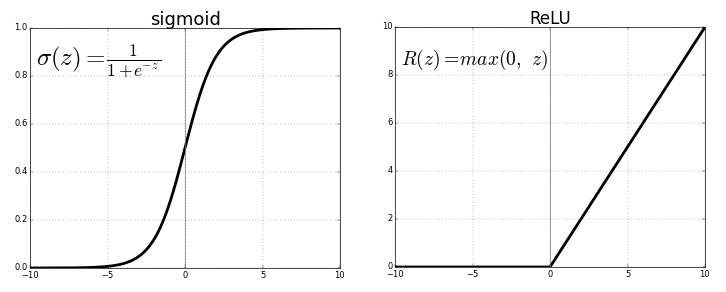
\includegraphics[trim={1cm 0 0 0 },clip,width=\linewidth]{sigmoid_relu.png}
       
        \tiny Quelle:~\url{https://towardsdatascience.com/activation-functions-neural-networks-1cbd9f8d91d6}
        \end{figure}
        
\end{columns}

\end{frame}


\begin{frame}\frametitle{Wdh. Knowledge Graph}
\begin{figure}
    \centering
    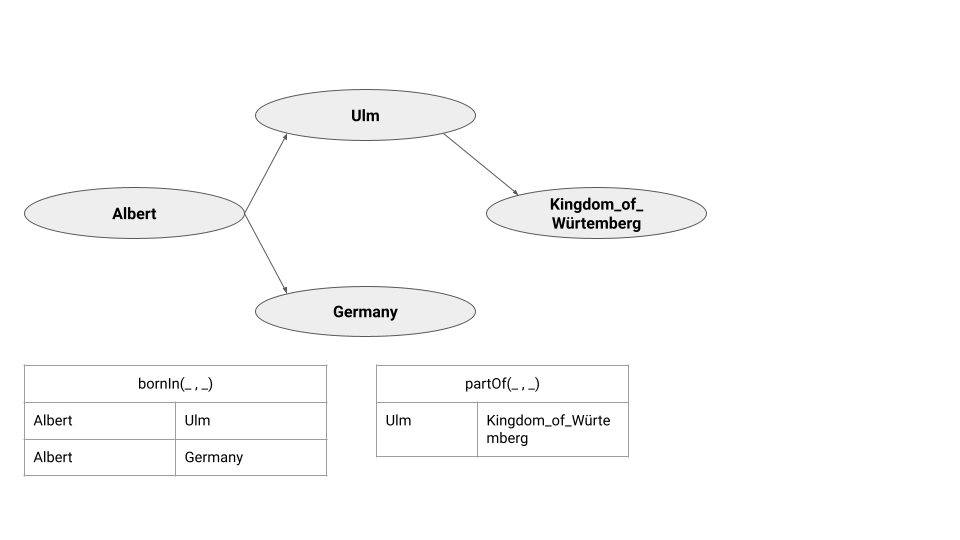
\includegraphics[width=0.73\textwidth]{1_LNN.png}
\end{figure}
\pause
\textcolor{red}{Was kann man schlussfolgern?}
\end{frame}

\begin{frame}\frametitle{Wdh. Knowledge Graph}
\begin{figure}
    \centering
    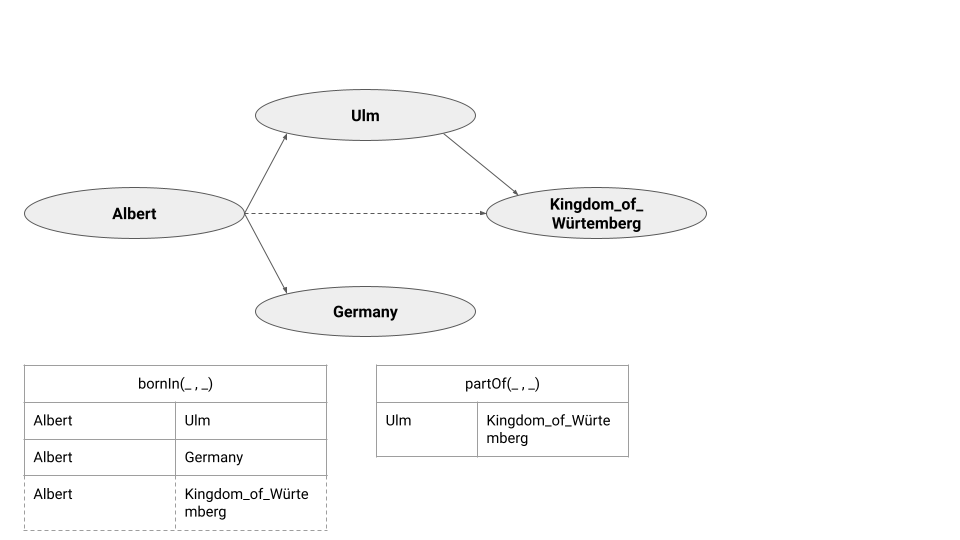
\includegraphics[width=0.73\textwidth]{2_LNN.png}
\end{figure}
\end{frame}

\begin{frame}\frametitle{Description Logic/First Order Logic Regeln}
\begin{figure}
    \centering
    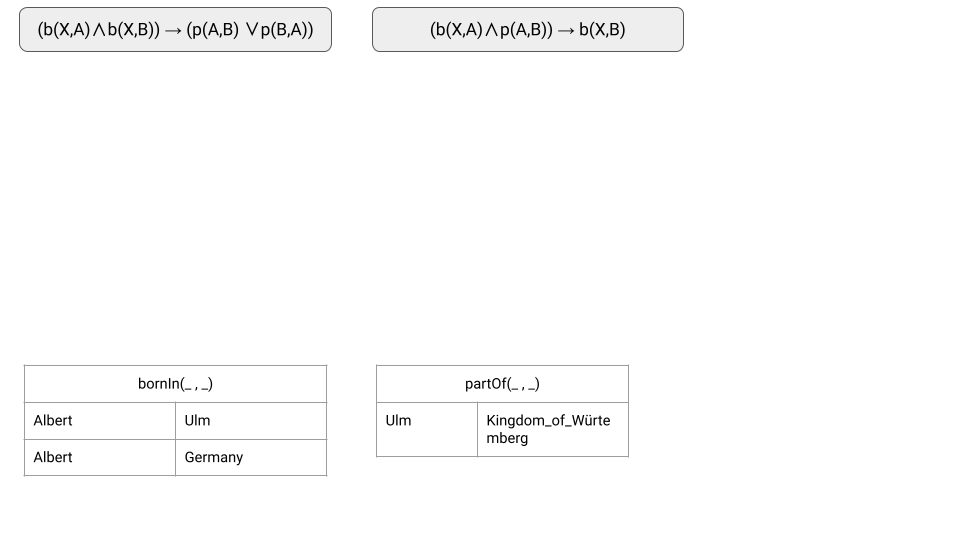
\includegraphics[width=0.73\textwidth]{3_LNN.png}
\end{figure}
\end{frame}

\begin{frame}\frametitle{Description Logic/First Order Logic Regeln - Syntaxbäume}
\begin{figure}
    \centering
    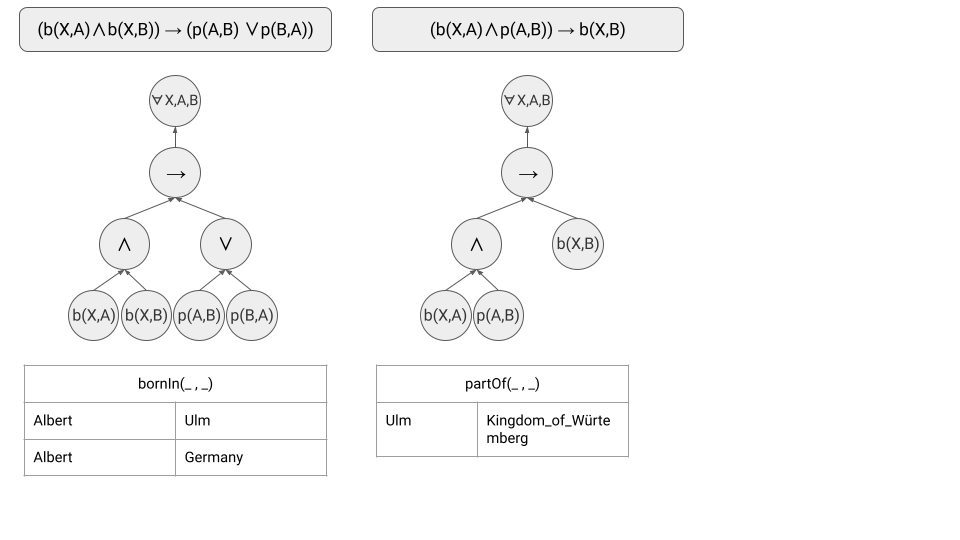
\includegraphics[width=0.73\textwidth]{4_LNN.png}
\end{figure}
\end{frame}

\begin{frame}\frametitle{Description Logic/First Order Logic Regeln - Wahrheitswerte}
\begin{figure}
    \centering
    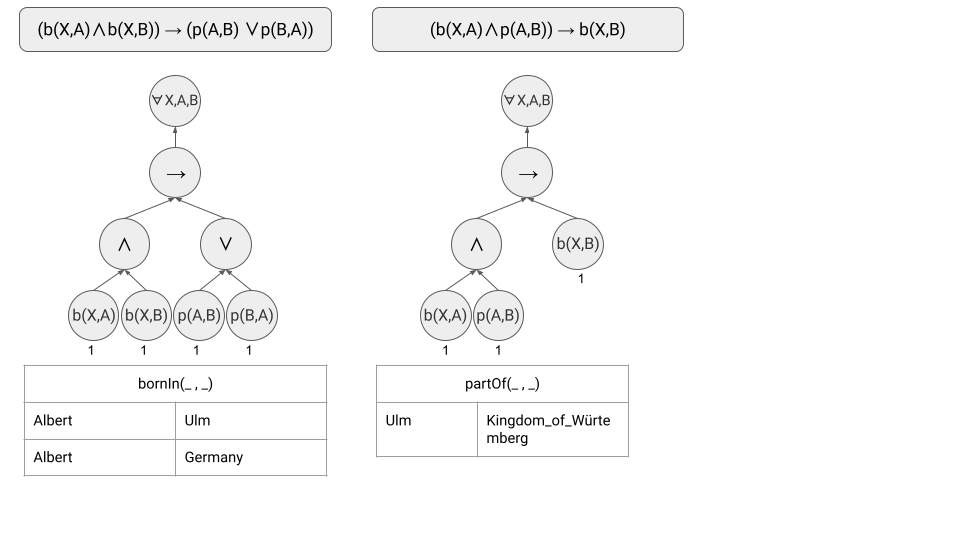
\includegraphics[width=0.73\textwidth]{5_LNN.png}
\end{figure}
\end{frame}

\begin{frame}\frametitle{Description Logic/First Order Logic Regeln - realwertige Wahrheitswerte}
\begin{figure}
    \centering
    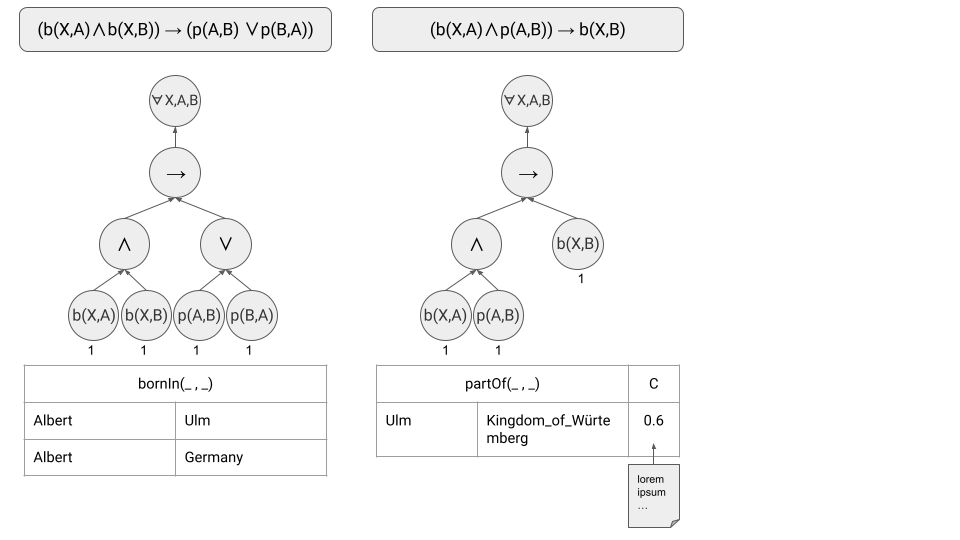
\includegraphics[width=0.73\textwidth]{6_LNN.png}
\end{figure}

\textcolor{red}{Warum reicht die mathematische Formulierung zur Modellierung von Konfidenzen nicht aus?}
\end{frame}

\begin{frame}\frametitle{Idee: Modelliere Logic mit Neuronalen Netzen (McCulloch und Pitts, 1943)}
\begin{columns}
    \column{0.4\textwidth}
        \begin{figure}
            \centering
            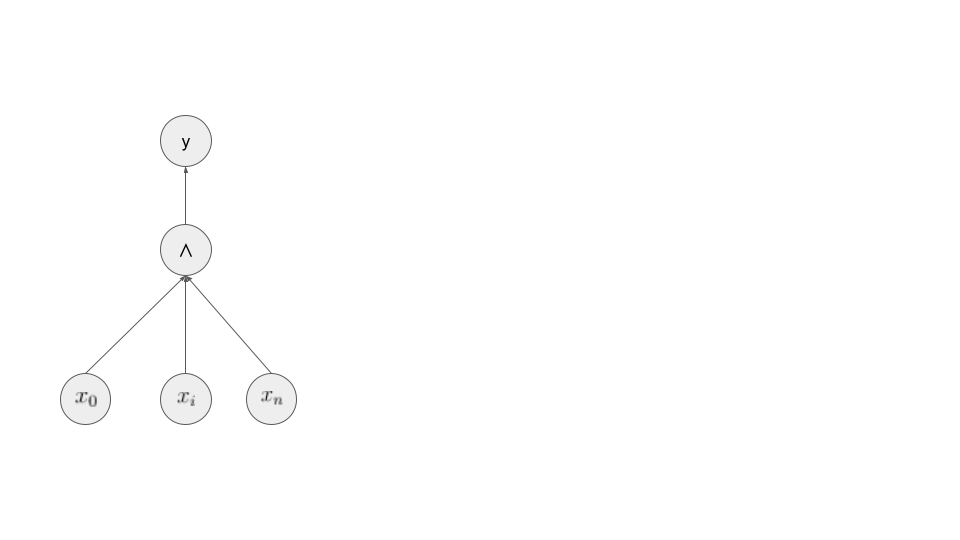
\includegraphics[trim={0 4cm 21cm 4cm },clip,width=\linewidth]{7_LNN.png}
        \end{figure}
        McCulloch-Pitts-Zelle

    \column{0.59\textwidth}
    \begin{itemize}
        \item Idee: Knoten werden zu Neuronen
        \item Input: $x_i \in \{0,1\}$
        \item Output: $y=step(\sum x - \theta)$
        \begin{figure}
            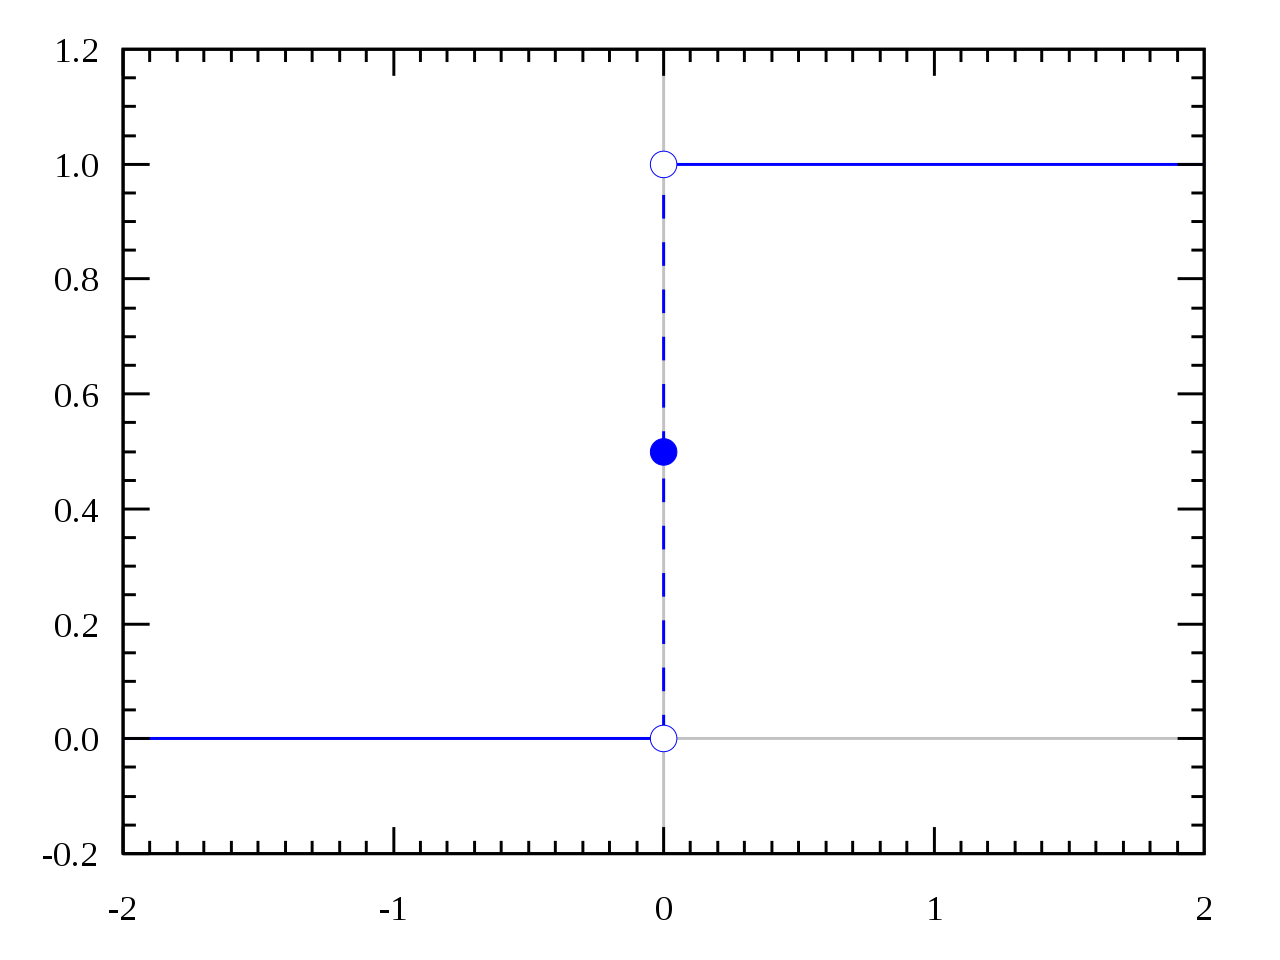
\includegraphics[width=0.4\linewidth]{step.png}
            %\tiny \textcolor{gray}{Quelle: \url{https://en.wikipedia.org/wiki/Heaviside_step_function\#/media/File:Dirac_distribution_CDF.svg}}
        \end{figure}
        \item Mathematische Verhalten:
        \begin{itemize}
            \item $p \wedge q = [\![ p+q > 1.5 ]\!]$
            \item $p \vee q = [\![ p+q > 0.5 ]\!]$
            \item $p \to q = [\![ 1-p+q > 0.5 ]\!]$
        \end{itemize}
    \end{itemize} 
        
    \pause
    \textcolor{red}{Was fehlt?}
\end{columns}
\end{frame}

\begin{frame}\frametitle{Idee: Logical Neural Networks (Riegel et al. 2020)}
\begin{columns}
    \column{0.4\textwidth}
        \begin{figure}
            \centering
            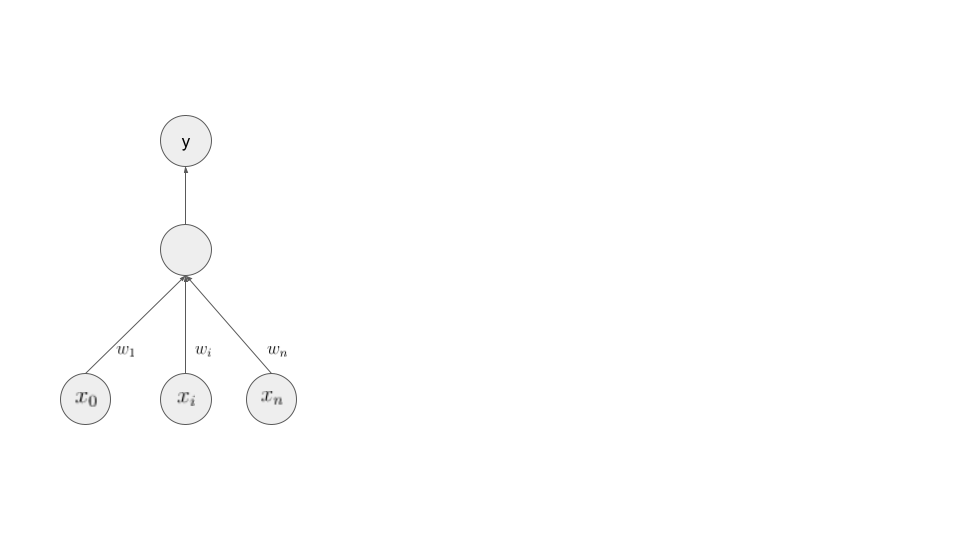
\includegraphics[trim={0 4cm 21cm 4cm },clip,width=\linewidth]{8_LNN.png}
        \end{figure}
    \column{0.59\textwidth}
    \begin{itemize}
        \item Ideen:
        \begin{itemize}
            \item Knoten werden zu Neuronen
            \item Kanten werden gewichtet
        \end{itemize}
        \item Input: $x_i \in [0,1]$
        \item Output: $y=f(w \cdot x - \theta)$ \textit{(Upward Inference)} 
        \begin{itemize}
            \item Mit $w_i,i, \theta \geq 0$
        \end{itemize}
      
        \item Einführung eines \textit{truth parameters} $0.5 < \alpha \leq 1.0$
        \begin{itemize}
            \item $p\geq \alpha $ interpretiert als wahr
            \item $p \leq 1 - \alpha$ interpretiert als falsch
        \end{itemize}
        \item $f$ ist eine monotone Aktivierungsfunktion
        \begin{itemize}
            \item $f(\alpha) = \alpha$
            \item $f(1- \alpha) = 1- \alpha$
        \end{itemize}
        \item Optimierung über \textit{Constrained Optimization} (nächstes Mal)
    \end{itemize} 
\end{columns}
\pause
\vspace{1mm}
\textcolor{red}{Was bringt uns das bezogen auf die Aussagekraft des Neurons?}
\end{frame}

\begin{frame}\frametitle{Idee: Logical Neural Networks (Riegel et al. 2020) --- Interpretierbarkeit}
\begin{columns}
    \column{0.4\textwidth}
        \begin{figure}
            \centering
            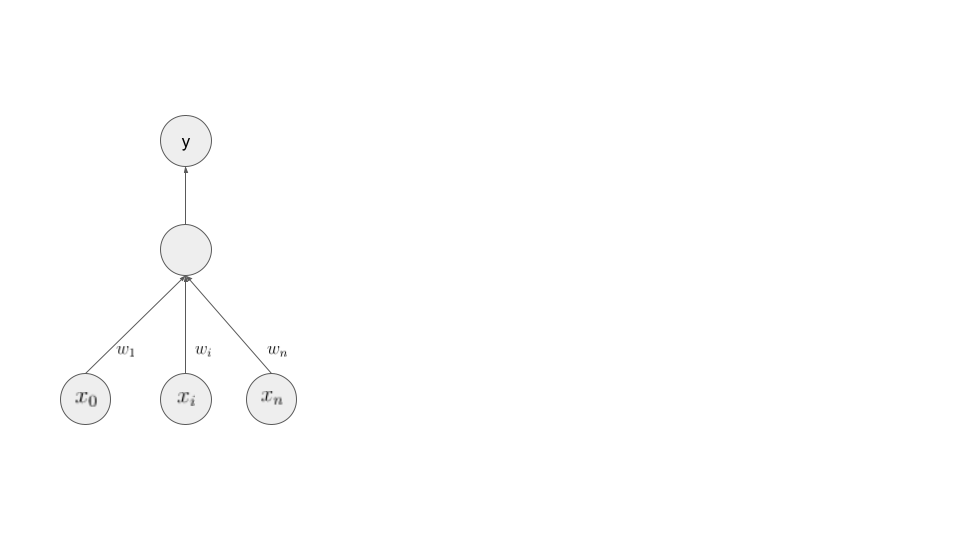
\includegraphics[trim={0 4cm 21cm 4cm },clip,width=\linewidth]{8_LNN.png}
        \end{figure}
    \column{0.59\textwidth}
        \begin{figure}
            \centering
            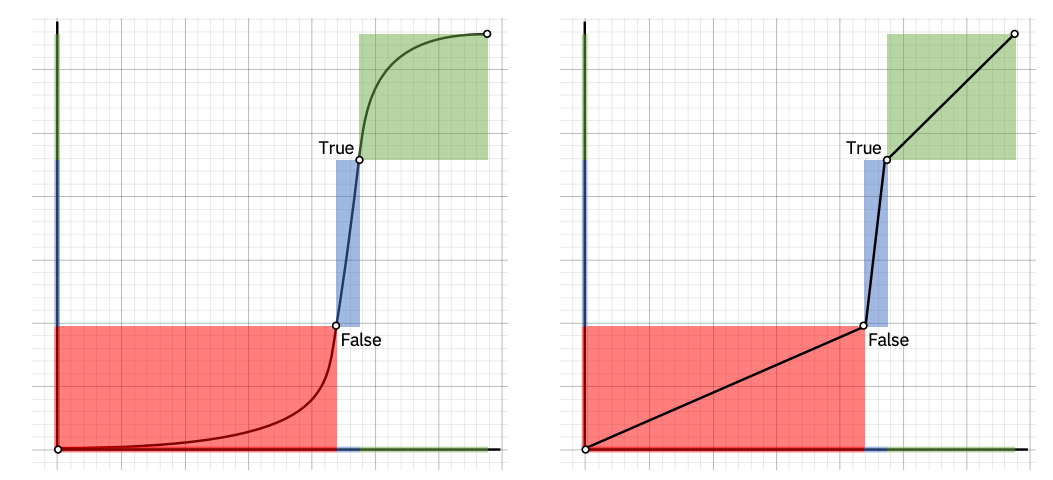
\includegraphics[width=\linewidth]{classical_region.png}
            \tiny \textcolor{gray}{Quelle: \url{https://arxiv.org/pdf/2006.13155.pdf}}
        \end{figure}
        \begin{itemize}
            \item Klassisches 'Und'-Verhalten 
            \begin{itemize}
                \item $\displaystyle \sum_i w_i \alpha \geq \alpha$ 'wahr'
                \item $\displaystyle \forall i \sum_j w_j - w_i \alpha - \theta \leq 1-\alpha $ 'falsch'
            \end{itemize}
        \end{itemize}
\end{columns}
\end{frame}




\begin{frame}[fragile]\frametitle{Logical Neural Networks (Riegel et al. 2020) - Überblick}
\textcolor{blue}{Idee:} Gewichte in Neuronalen Netzen können als logische Funktionen interpretiert werden
\begin{itemize}
    \item \textbf{Neuron}: Repräsentiert ein Element in einer Logischen Formel (entweder Variable oder Operator) mit Gewichten an den Verbindungen
    \item \textbf{Training}: Feature-Value-Paare  
    \item \textbf{Auswertung}: erfolgt über monotone Verschärfung unterer und oberer Schranken von Subformeln in einem \textit{upward/downward pass} über den Syntaxbaum (nächstes Mal)
    %\item (Ähnlichkeit zu Recurrent-Neural-Networks)
    \item \textbf{Eigenschaften}: E2E-differenzierbar, deterministisch, Widersprüche abbildbar, \textit{Open World Assumption}, \textit{disentangle} Repräsentation
    \item[$\Rightarrow$] Modularität führt zu Generalisierbarkeit
\end{itemize}
\end{frame}

%modus ponus, if you know a, and a implies b, you know b
% Message passing

\begin{frame}\frametitle{Logical Neural Networks (Riegel et al. 2020) - Beispiel}
\begin{figure}
    \centering
    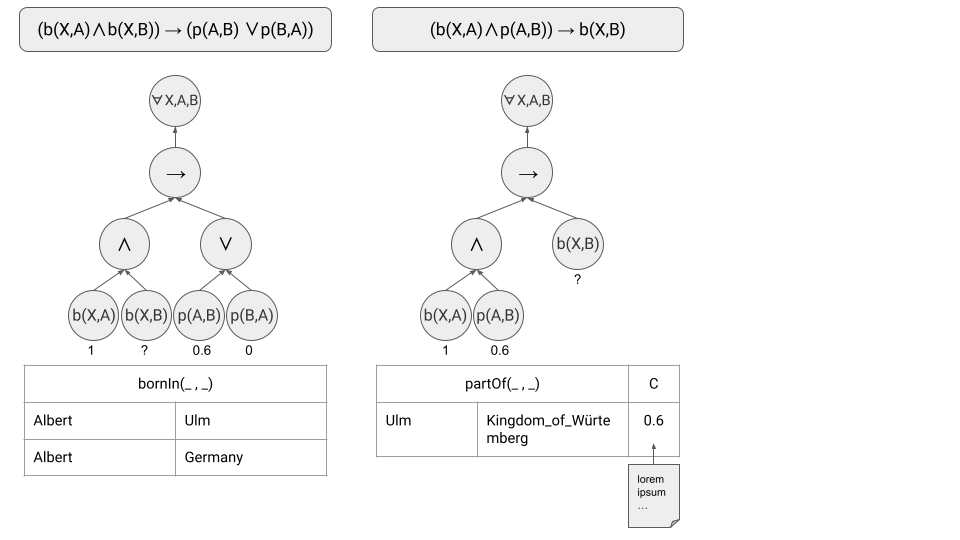
\includegraphics[width=0.73\textwidth]{9_LNN.png}
\end{figure}
\end{frame}

\begin{frame}\frametitle{Logical Neural Networks (Riegel et al. 2020) - Beispiel}
\begin{figure}
    \centering
    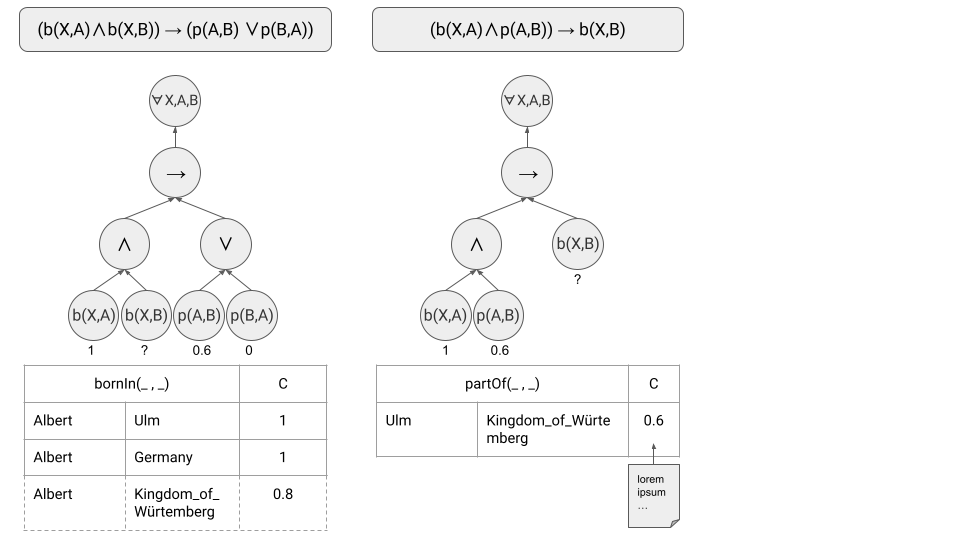
\includegraphics[width=0.73\textwidth]{10_LNN.png}
\end{figure}
\end{frame}

\begin{frame}\frametitle{Warum eine Kombination von statistischen Lernverfahren und Logik?}
Symbolische Systeme:
\begin{exampleblock}{Eigenschaften}
    \begin{itemize}
     \item - Hoher manueller Aufwand
     \item + \textit{Compositional Generalizability}
    \end{itemize}
\end{exampleblock}
Sub-symbolische Systeme und statistische Lernverfahren (z.B. Deep Learning):
\begin{exampleblock}{Nachteile}
    \begin{itemize}
        \item + Starke Performance, wenn genügend Trainingsdaten verfügbar
        \item - Keine Interpretierbarkeit
    \end{itemize}
\end{exampleblock}
Lösung: Hybride Künstliche Intelligenz (bspw. mit Logical Neural Networks)!

\vspace{3mm}
\tiny \textcolor{gray}{Mehr lesen: Garcez, Artur d’Avila, et al. "Neural-symbolic learning and reasoning: A survey and interpretation." Neuro-Symbolic Artificial Intelligence: The State of the Art 342 (2022)}
\end{frame}
 
 
\begin{frame}\frametitle{Logical Neural Networks (Riegel et al. 2020) - Anwendungen}
\begin{figure}
    \centering
    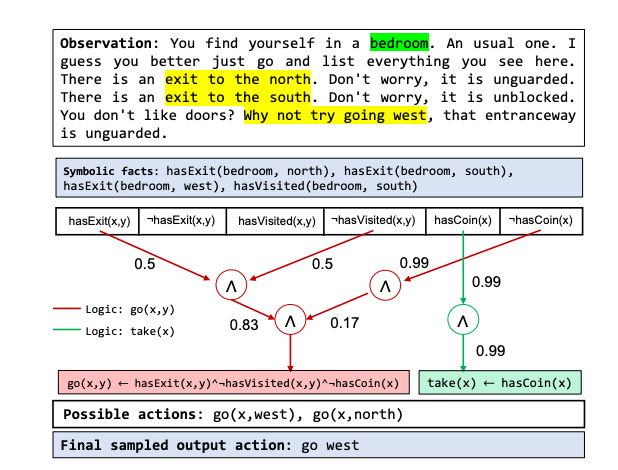
\includegraphics[width=0.5\linewidth]{Neuro-Symbolic Approaches for Text-Based Policy Learning.png}
    
    \tiny Quelle: Chaudhury, Subhajit, et al. 'Neuro-Symbolic Approaches for Text-Based Policy Learning.' Proceedings of the 2021 Conference on Empirical Methods in Natural Language Processing. 2021. 
\end{figure}

Aber auch bei Entity Linking, Question Answering (NSQA SOTA on QALD-9), ...
%Fall Beispiel QA 
%Leaderboard QA https://kgqa.github.io/leaderboard/dbpedia/qald.html#qald-9
%https://towardsdatascience.com/nsqa-neuro-symbolic-question-answering-6d14d98e88f3 
%https://arxiv.org/pdf/2012.01707.pdf
\end{frame}


\begin{frame}[fragile]\frametitle{Logical Neural Networks (Riegel et al. 2020) - Code}
    \begin{columns}
	\column{.59\textwidth}
	 \begin{center}
        \begin{itemize}
            \item Inferenz erzeugt:
            \item[]
            \begin{verbatim}
('Albert', 'Ulm', 'Kingdom_of_Wuertemberg') 
    APPROX_TRUE (0.6, 1.0)
            \end{verbatim}
        \end{itemize}
    \end{center}
	\column{.4\textwidth}
        \begin{figure}
        \centering
        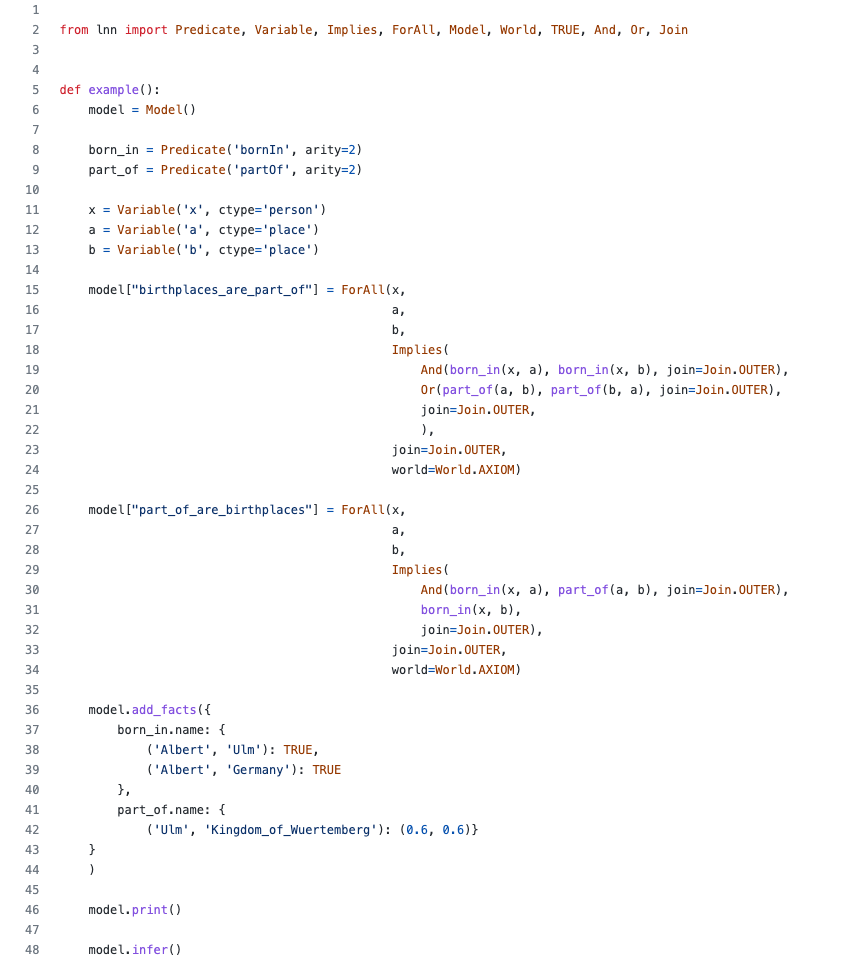
\includegraphics[width=0.95\linewidth]{code.png}
       
        \tiny Quelle:~\url{https://github.com/RicardoUsbeck/HI} 
        
        Kudos to C. Möller
        \end{figure}
    \end{columns}
\end{frame}

\begin{frame}{Take-Away und Ausblick} 
Was haben wir gelernt?
\begin{itemize}
    \item Grundaufbau Logische Neuronale Netze
    \item Vorteile Hybrider KI
\end{itemize}
Wo können wir weiter lernen oder ausprobieren?
\begin{itemize}
    \item Original Code: \url{https://github.com/ibm/lnn}
    \item Beispiel Code: \url{https://github.com/RicardoUsbeck/HI}
\end{itemize}
Was passiert beim nächsten Mal?
\begin{itemize}
    \item Bidirektionale Inferenz: modus ponens, modus tollens
    \item Optimierung von LNNs
\end{itemize}
Was sollte man bis zum nächsten Mal gelesen haben?
\begin{itemize}
    \item Lesen: \url{https://ibm.github.io/LNN/}
\end{itemize}
\end{frame}


%%%% REFERENZEN %%%%
\begin{frame}\frametitle{Quellen}
\begin{itemize}
    \item Riegel, Ryan, et al. 'Logical neural networks.' arXiv preprint arXiv:2006.13155 (2020).
    \item Fagin, Ronald, Ryan Riegel, and Alexander Gray. "Foundations of reasoning with uncertainty via real-valued logics." arXiv preprint arXiv:2008.02429 (2020).
    \item McCulloch, Warren S., and Walter Pitts. "A logical calculus of the ideas immanent in nervous activity." The bulletin of mathematical biophysics 5.4 (1943): 115-133.
    \item Blog - \url{https://skirmilitor.medium.com/logical-neural-networks-31498d1aa9be}
    \item Youtube - KRHCAI Invited Talk by Alexander Gray: Logical Neural Networks \url{https://www.youtube.com/watch?v=m687EBE0Nqw}
\end{itemize}
\end{frame}


\begin{frame}{\textbf{Danke für Ihre Aufmerksamkeit!}}
    \begin{columns}
	\column{.59\textwidth}
	 \begin{center}
        \small{\faGraduationCap \hspace{0.15em} {Lernmaterial (VL, Selbsttests, Übungen, Links zu Jupyter Notebooks...)\\\small{\faGithub \hspace{0.15em} {\href{https://github.com/RicardoUsbeck/HI}{http://github.com/RicardoUsbeck/HI}}}}} \\
        \smallskip
        \Huge {Welche Fragen haben Sie?} \\
        
    \end{center}
	\column{.4\textwidth}
	\centering
	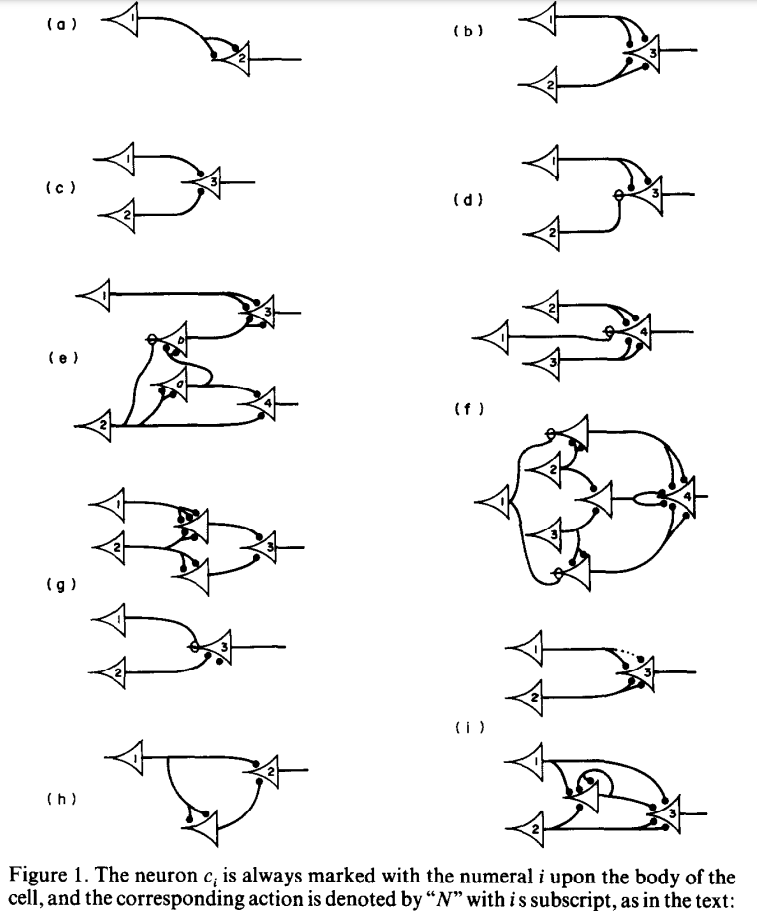
\includegraphics[width=0.7\linewidth]{mcculloch.png}\\
	
	\vspace{5mm}
	
	\tiny \textcolor{gray}{Quelle: McCulloch, Warren S., and Walter Pitts. 'A logical calculus of the ideas immanent in nervous activity.' The bulletin of mathematical biophysics 5.4 (1943): 115-133. \url{https://www.cs.cmu.edu/~./epxing/Class/10715/reading/McCulloch.and.Pitts.pdf}}

\end{columns}
\end{frame}


%\begin{frame}[fragile]\frametitle{Bonus: Entstehung Logischer Neuronen:  McCulloch und Pitts Neuron 1943}
%\begin{figure}
%    \centering
%    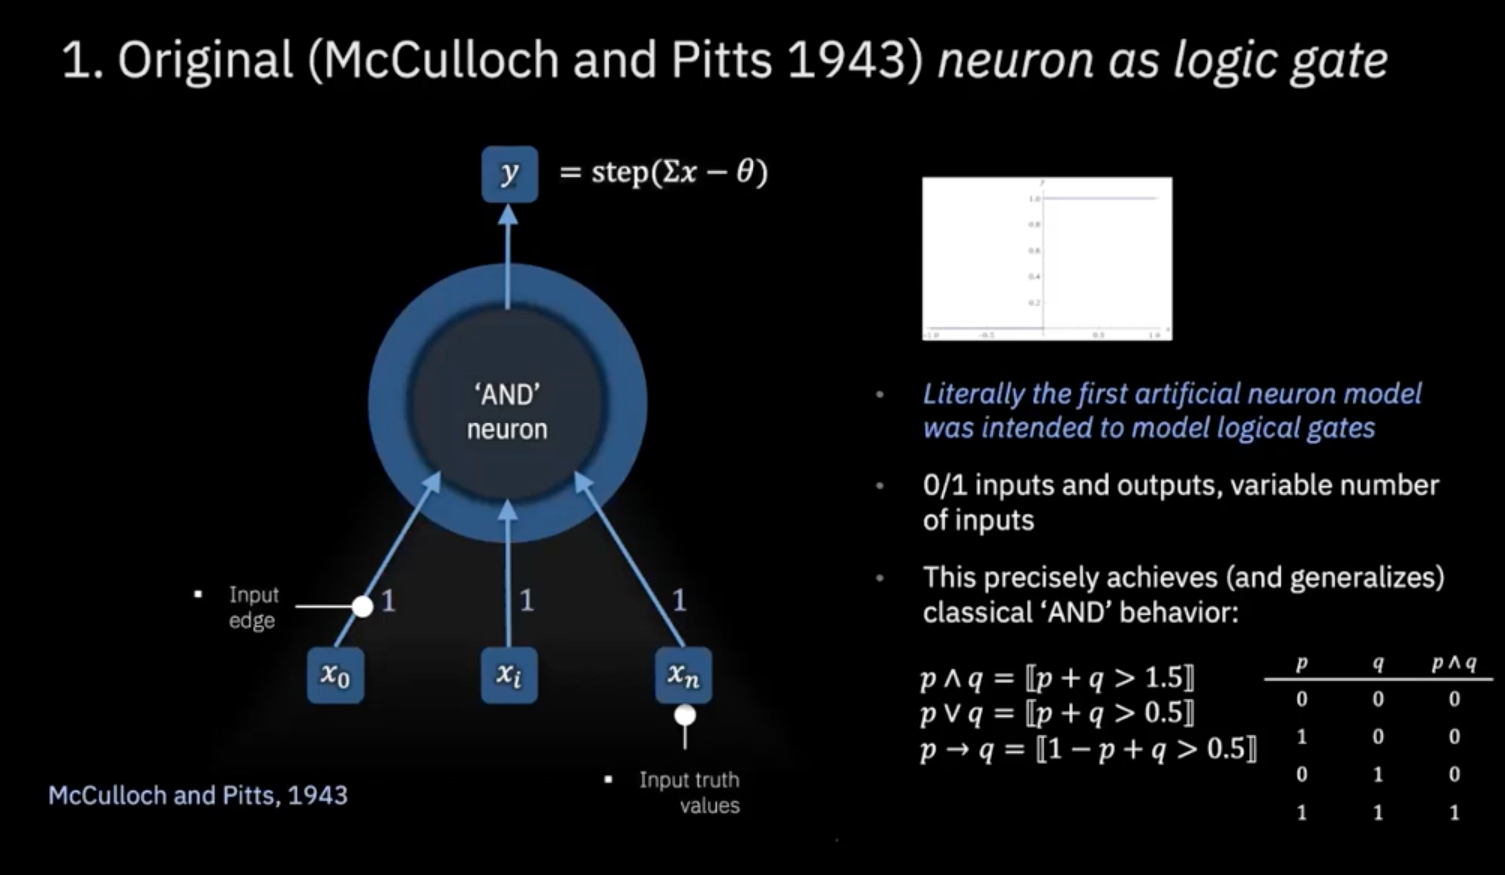
\includegraphics[width=0.7\linewidth]{mcculloch_neuron.png}
   
%    \tiny Source:~\url{https://www.youtube.com/watch?v=kAaKs_04dEk&ab_channel=CenterforScienceofInformationNSFSTC}
%\end{figure}
%\end{frame}


\begin{frame}[fragile]\frametitle{Bonus: Łukasiewicz Logik als Basis}
\textcolor{blue}{Definition:}  
\begin{itemize}
    \item Grundannahme, dass 'unknown implies unknown' wahr ist is true
    \item $p \bigotimes q = max (0,p+q-1)$ (and)
    \item $p \bigoplus q = min (1,p+q)$ (or)
    \item $p \to q = min (1,1-p+q)$ (or)
    \item If you plot this, it looks like ReLu!
    \item But (!) it does not allow for real-valued inputs
\end{itemize}
\end{frame}
 
\begin{frame}\frametitle{Bonus: Logical Neural Networks (Riegel et al. 2020) - Eigenschaften}
\begin{itemize}
    \item LNNs sind \textit{End-to-End differenzierbar} 
    \item Inferenz ist \textit{omnidirektional} und \textit{deterministisch}, d.h. Relationen sind bidirektional inferierbar und Herleitungen wiederholbar
    \item Inferenz konvergiert beweisbar in endlicher Anzahl Schritte
    \item \textit{Loss-Function} bildet auch logische Widersprüche ab
    \item LNNs arbeiten mit der \textit{Open World assumption}% , d.h. Variablen sind nicht wahr oder falsch sondern haben obere und untere Wahrheitsschranken (im Gegensatz zu Markov Random Fields) $\Rightarrow$ Probabilistische Semantik
    \item Formeln sind \textit{modular} und \textit{compositional}, d.h. es kann hierarchische Beziehungen für Formeln geben
    \item Representation ist \textit{disentangeled}, d.h. es gibt nicht einen einzigen Vektor für die Formel
\end{itemize}
\end{frame}
 
\end{document}
